\chapter{Characterization}

\subsection{Intro}
Our work focuses on characterizing the energy and latency of end-to-end Omni-directional(OD) Camera  systems. The goal is to find the bottlenecks of different components in the hardware and software pipeline and propose optimizations. As the existing OD camera systems are built from off the shelf camera devices and uses the conventional stitching algorithms we see a potential research opportunity to close gaps between hardware and software. Many existing systems like Google Jump, Facebook Surround capture and compute on enormous amount of data consuming several hundreds of watts of power to stitch images in realtime 30fps. The main challenge in OD panorama generation is to understand the data flow across the system and to make decisions on data abstractions needed at different subcomponents to reduce the total system power.

Many have argued [Edvardo Hotmobile, Nvidia, AMD] that we need resolutions greater than 16k and frame-rate greater of 240 for true immersion in VR. At such higher framerate and resolutions there is lot of information that is redundantly captured, processed and transferred. Therefore, in our work, we study how the energy and latency of each stage get affected by the output resolution and the characterize the bottlenecks in greater detail. 

We characterize both monoscopic and ODS camera systems. The difference between them is the number of novel views needed is significantly higher for ODS. Monoscopic is a special case of ODS and at core involves the same optical flow based stitching. So we will characterize generalized flow based stitching system and notify any important differences between monoscopic and ODS when necessary.\newline

\section{Prototype System Overview}

The end to end camera system, as shown in figure 3.1 can be divided into 4 major stages by energy consumption, viz., image sensor, image signal processor(ISP), processor, and Off-chip memory. For our prototype camera design we use six IMX-274 cameras for capture and Nvidia Jetson TX2 for supporting camera capture and processing. The Camera and Jetson specs are shown in figure 3.2. 

Prototype System Overview\newline
Hardware:
System 1) Six Camera Rig for OmniDrirectional Stereo\newline
System 2) Dual Fisheye Camera for monoscopic 360 \newline
Software:
Nvidia libargus Camera API,
openCV, C++ \newline

\section{Energy and Latency Measurement Methodology}
Jetson has power monitor IC and ways to moniter CPU, GPU, memory frequencies. We measure the absolute energy of the system and the difference between the idle and active state for individual stages of the pipeline.
Measurement by experiments:
Jetson power monitor for camera and ISP, and Optical flow power from Zynq\newline
Analytical and Simulation based:
Micron System Power Calculator for LPDDR2. \newline
Application run time measurement.




\section{Energy Characterization}
\subsection{Individual stage energy}
	\begin{tabular}{c|c|c|c}
	Power Rail & Diff. Current(mA) & Voltage(mV) & Energy ( mJ/frame) \\
	Camera & 375.4 & 3336 & 41.7 \\
	ISP+CODEC & 102.7 & 19152 & 65.6 \\
	CPU & 16.4 & 19144 & 10.5 \\
	DDR & 260.4 & 4792 & 41.6 \\
	Stitch[CPU] & [] & [] & [] \\
	\end{tabular} \newline \newline
	The camera system is configured to 1920x1080 resolution at 30 fps for the below measurements. [make absolute energies instead of diff. i.e active -idle]\newline
	
	As seen in the above table, the processing  the optical flow implementation in software is expensive both in terms of energy and latency. Therefore, we approximate the energy and latency for FPGA based accelerator based on Xilinx's implementation of optical flow on Zynq board, discussed in chapter5.\newline

	
\section{Characterization Results - Latency}

 Performance \newline
	a) Individual Stage Latency Characterization
	
	% Breakdown of sharpening \newline

\subsection{Individual Stage latency}
For camera system and ISP stages the latency is taken from NVIDIA camera API documentation. We measure the latency of computation in terms of CPU runtime. 

\subsection{Optical flow runtime breakdown}
Time for each Pyramid search(98\%) as shown in fig 3.1.
\begin{figure*}
	\begin{center}
		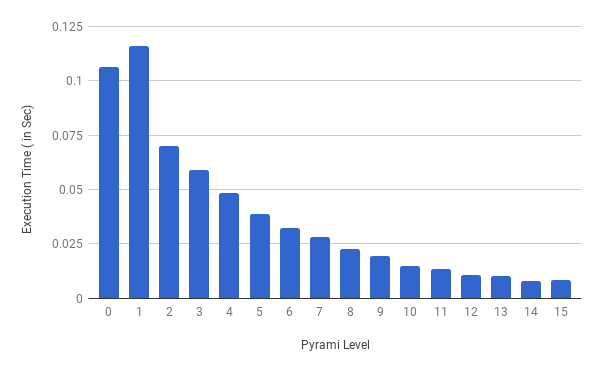
\includegraphics[width=1\textwidth]{/media/gunman/Data/thesis/ThesisLatex/data/images/pyramid_runtime.png}
		\caption{X-axis shows the pyramid level and Y-axis the runtime tile search and propagate.}
		\label{fig:ex_4_9}
	\end{center}
	\vspace{-0.3in}
\end{figure*} 

\subsection{Sensor Response Time}
Camera startup time needs to be less. 
	Initial frames are low contrast but improves over time. 
	% May be regenerate these figures
	%/media/gunman/Data/Programming/python_coding
	\begin{figure*}
		\begin{center}
			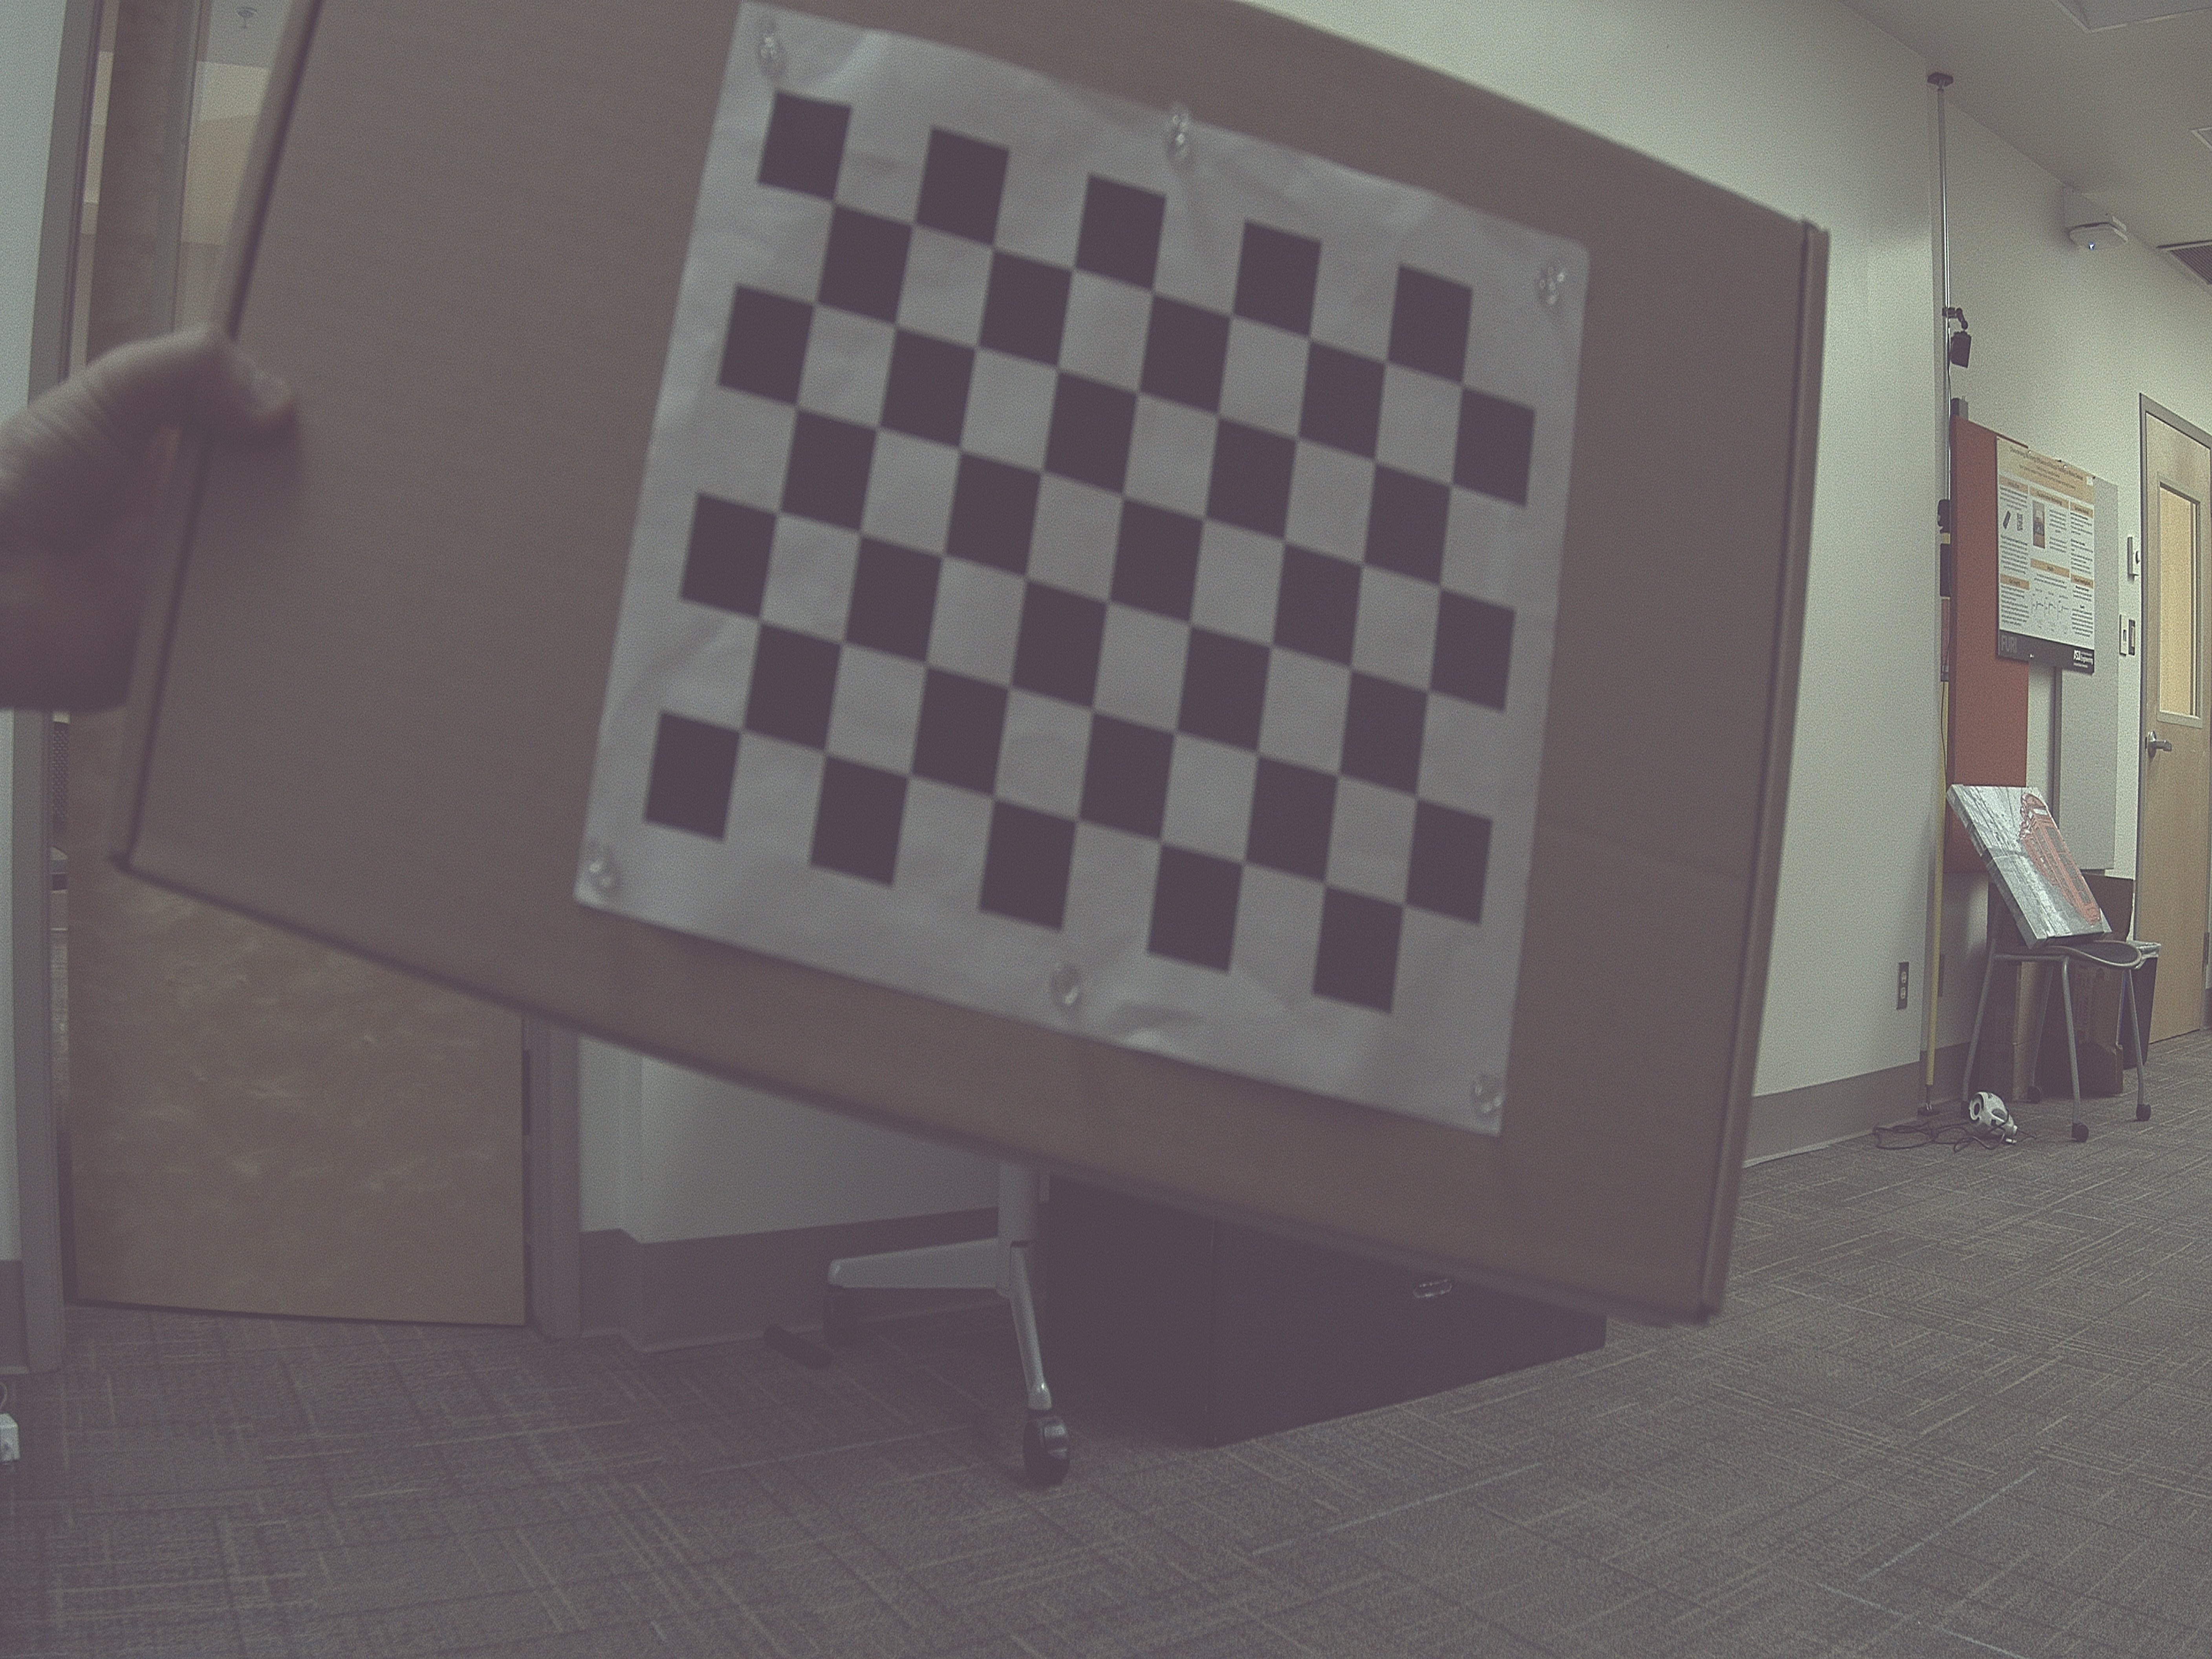
\includegraphics[width=1\textwidth]{/media/gunman/Data/thesis/ThesisLatex/data/images/sensor0_low_contrast.jpg}
			\caption{X-axis shows the pyramid level and Y-axis the runtime tile search and propagate.}
			\label{fig:ex_4_9}
		\end{center}
		\vspace{-0.3in}
	\end{figure*} 

	\begin{figure*}
	\begin{center}
		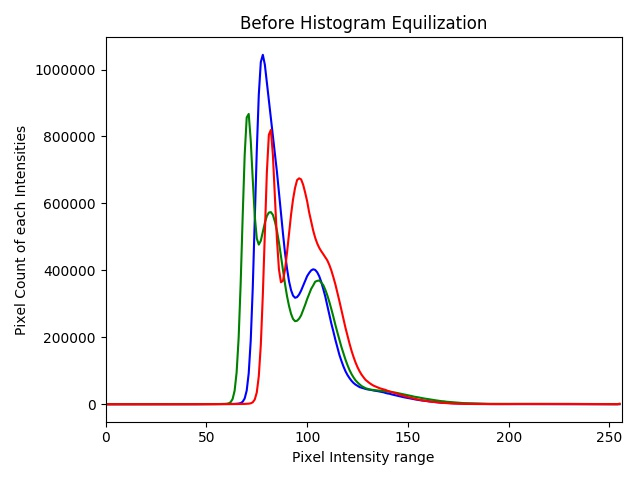
\includegraphics[width=1\textwidth]{/media/gunman/Data/thesis/ThesisLatex/data/images/Before_Histogram_equilization.jpg}
		\caption{X-axis shows the pyramid level and Y-axis the runtime tile search and propagate.}
		\label{fig:ex_4_9}
	\end{center}
	\vspace{-0.3in}
\end{figure*} 

	\begin{figure*}
	\begin{center}
		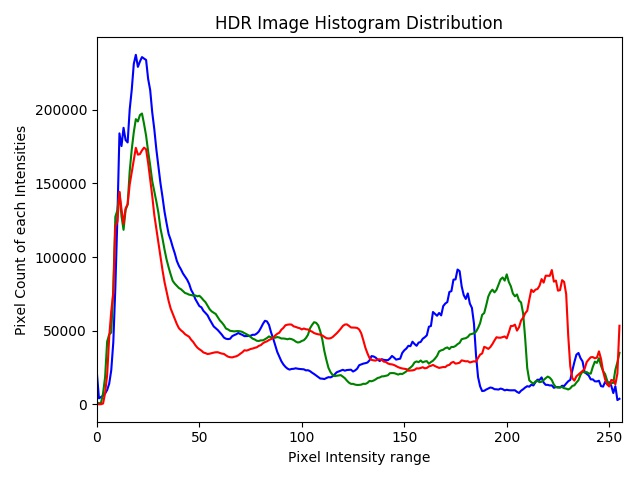
\includegraphics[width=1\textwidth]{/media/gunman/Data/thesis/ThesisLatex/data/images/Normal_Histogram_Distribution.jpeg}
		\caption{Xaxis shows the pyramid level and Y-axis the runtime tile search and propagate.}
		\label{fig:ex_4_9}
	\end{center}
	\vspace{-0.3in}
\end{figure*} 


\section{Design Scalability}	

\subsubsection{Runtime scalability with the resolution}
Outputs:
4k, 6k, 8k, 12k
Discuss scalability of resolution for different stages. \newline
Especially the scalability of cache, DRAM, CPU power. 
\begin{figure*}
	\begin{center}
		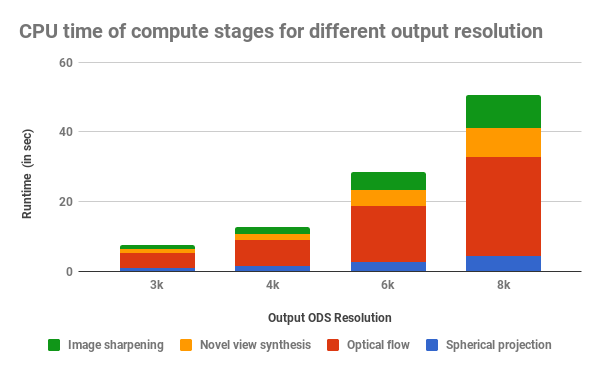
\includegraphics[width=1\textwidth]{/media/gunman/Data/thesis/ThesisLatex/data/images/ExecutionTimeComputeStages.png}
		\caption{CPU execution time of different compute stages. X axis has different sub-stages in optical flow and Y axis correspond to energy per frame.}
		\label{fig:ex_4_9}
	\end{center}
	\vspace{-0.3in}
\end{figure*} 

What is the energy per each output pixel	
What is energy per pixel when generating only one ODS view, and how does it compare when generating two views! If it is double then we have a problem to solve	
[Check why sharpening is so costly!]

\subsubsection{Resource scalability with the resolution}
We measure the DRAM capacity required and bandwidth needs as we increase the resolution as a parameter for resource scalability. Higher capacity indicates the need for better encoding schemes and high bandwidth can indicate the temporal redundancy in the data, thereby increasing the bandwidth. For 3k, 4k, 6k and 8k output resolution.

Although we built a system where all the cameras are capturing at same resolution and framerate at a given time, we expect the future cameras make these decisions dynamically to save power. Therefore, we  measure the efficiency of capture and ISP processing at different modes of operation and measure the efficiency of capture and processing in power consumed per pixel at different modes.

DRAM memory size\newline
\begin{tabular}{c|c|c|c|c}
	Stage & 3k & 4k & 6k & 8k \\
	camera Input & - & - & - & - \\
	ISP & - & - & - & - \\
	Motion Estimation & - & - & - & - \\
	fish2EqRect Projection & - & - & - & - \\
	Optical Flow & - & - & - & - \\
	Sharpen & - & - & - & - \\
\end{tabular} 

\vspace{10mm}
\begin{tabular}{c|c|c|c|c}
	o/p Resolution & 3k & 4k & 6k & 8k \\
	Avg. DRAM BW & - & - & - & - \\
\end{tabular} 
\vspace{30mm}

% Figure 
\begin{figure*}
	\begin{center}
		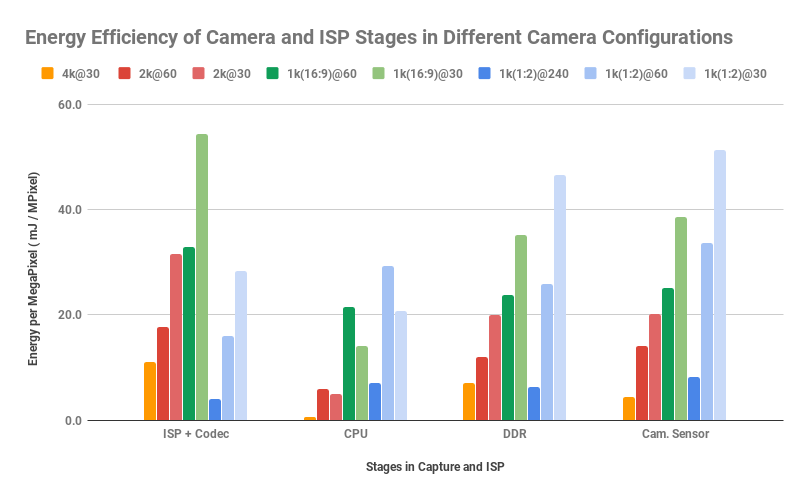
\includegraphics[width=1\textwidth]{/media/gunman/Data/thesis/ThesisLatex/data/images/Power_Efficiency_of_Camera_ISP_Stages_in_different_configurations.png}
		\caption{Power Efficiency of Camera ISP Stages in different configurations}
		\label{fig:ex_4_9}
	\end{center}
	\vspace{-0.3in}
\end{figure*} 

Static and Dynamic Power. Resourse Utilization. 
Clock gating:
We were able to do clock gating of pixel clock. It works fine. The next step is to select between multiple clocks and see how it affect the output image.

Latency:
By varying the latency of reconfiguration, the image is not stable. It shows horizontal and vertical bars of image. This has to be fixed in this week. 


\section{Evaluating data-flow redundancies}
Evaluating redundant computations in optical flow. 
Accuracy Vs Energy\&Perf tradeoff. 
Next we evaluate the optical flow for a scene where foreground has movement and background is static. The temporal flow difference is found out to see the variation of flow. As expected we see the flow change only for the regions where the objects are moving. This observation suggests that accuracy of optical flow can be trade-off with computation time to save energy and latency. It also shows that the accuracy drop is less than \_ percent which can be acceptable


\section{Misc}

	
Increased frame-rate\newline
What is the percentage of new data
ffmpeg I-frame size to the P-frame ratio.
\begin{figure*}
	\begin{center}
		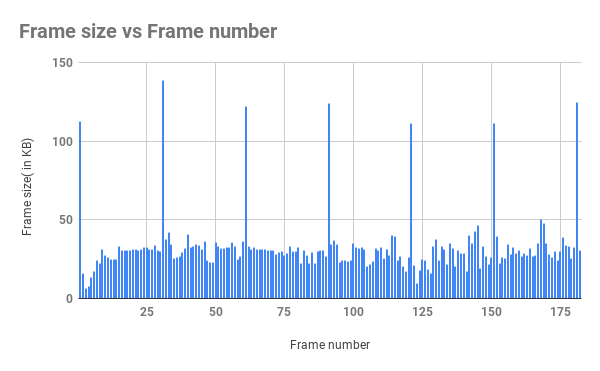
\includegraphics[width=1\textwidth]{/media/gunman/Data/thesis/ThesisLatex/data/images/FramesizevsFramenumber.png}
		\caption{Framesize of I and P frames}
		\label{fig:ex_4_9}
	\end{center}
	\vspace{-0.3in}
\end{figure*} 
%ffprobe lab.mp4 -show_frames
we usually have I,P, and B frames in a compressed video, but in case of realtime compression we will have only I and P frames and disable B frames as it adds latency to the pipeline. Typically I-frame to P-frame is about ~4 times and one I-frame occur for ~30 P-frames. This implies we save a lot on interface power if we can push the computation to near sensor.  
[Numbers - savings from IO datarate reduction]

3) Survey of Camera and ISP stage energy breakdown
Camera Sensor and ISP power directly taken from literature.
Computation Power split into sub stages. \newline
For power characterization of camera sensor and ISP, we run the camera in different resolutions and framerates and see how the various sub-component power changes. The components include Camera Sensor, I/O, ISP, CODEC, DDR, and CPU. The ISP, and CODEC power are combined as they belong to same SOC voltage rail.

The most used configuration for our project when all the six cameras are capturing 1920x1080 @ 30 fps. At this configuration below is the split of different component power. \newline


	e) Quality Tradeoff's with input resolution\newline
Sharpening
Reduction in fidelity of unwarped image, as interpolation is not being done.
Reducing number of pyramid's
f) High motion Vs low motion differences. Size of motion vector to that of size of full frame. 
g) File IO power
h) Breakdown in terms of type of Memory	used
i) Breakdown in terns of type of Computation
j) Breakdown in terms of IO bandwidth bottlenecks